\section{Background: Time Series Classification using Untrained Convolutional Kernels}
\label{sec:Background}

We describe a family of time series classifiers which take inspiration from \textbf{random convolutional kernels} in machine learning \cite{Jarrett2009, Pinto2009, Cox2011, Saxe2011, Yosinski2014}: a large number of randomly-generated kernels with fixed weights can capture many relevant features for a downstream classifier. This approach is quite different from \textbf{convolutional neural networks (CNNs)} where kernel weights are learned \cite{Cui2016, Wang2017, Fawaz2019a, Fawaz2019b, Zimmerman2019, InceptionTime, Fawaz2020b}. We describe key components which are common to convolutional kernel-based time series classifiers and then specify four classifiers using this framework. 

\subsection{Classifier Overview}
\label{sec:Overview}

Let $T = \langle t_1, t_2, \ldots, t_n \rangle \in \mathbb{R}^n$ be a time series of length $n$. $T$ can be \textbf{padded} with leading/trailing zeroes as needed. $T$'s \textbf{first-order difference}, $T' = \langle t_i - t_{i-1}| 2 \leq i \leq n \rangle \in \mathbb{R}^{n-1}$, is also a time series (e.g., see Fig. \ref{fig:first_order_difference}). 

\begin{figure}[tp]
    \centering
    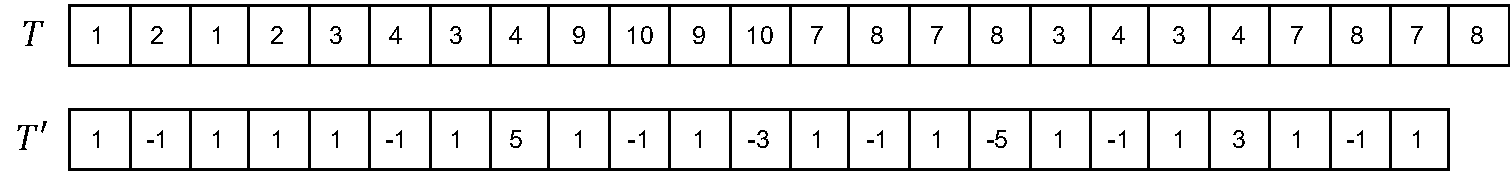
\includegraphics[width=\linewidth]{Figures/first_order_difference.pdf}
    \caption{A time series $T$ and its first-order difference series $T'$.}
    \label{fig:first_order_difference}
\end{figure}

Let $\omega \in \mathbb{R}^m, m \ll n$ be an ordered sequence of constant values called a \textbf{kernel}. Kernel values are either randomly generated or chosen by the classifier designer. A \textbf{feature map} $T * \omega \in \mathbb{R}^{n-m+1}$ is computed by applying a one-dimensional \textbf{convolution} operator $*$ to $T$ and $\omega$. A convolution $*_d$ with a \textbf{dilation} of $d$ skips every $d-1$ scalar elements of $T$ during the convolution \cite{Yu2015, Bai2018}, e.g., $*_1$ is a standard convolution, $*_2$ skips every-other element of $T$, etc.; when accounting for dilutions $T *_d \omega \in \mathbb{R}^{(n-m+1)/d}$.
We further discuss dilutions in Section \ref{sec:Dilations}. Fig. \ref{fig:convolutions} illustrates these concepts.

\begin{figure}[tp]
    \centering
        \begin{subfigure}{\linewidth}
      \centering
      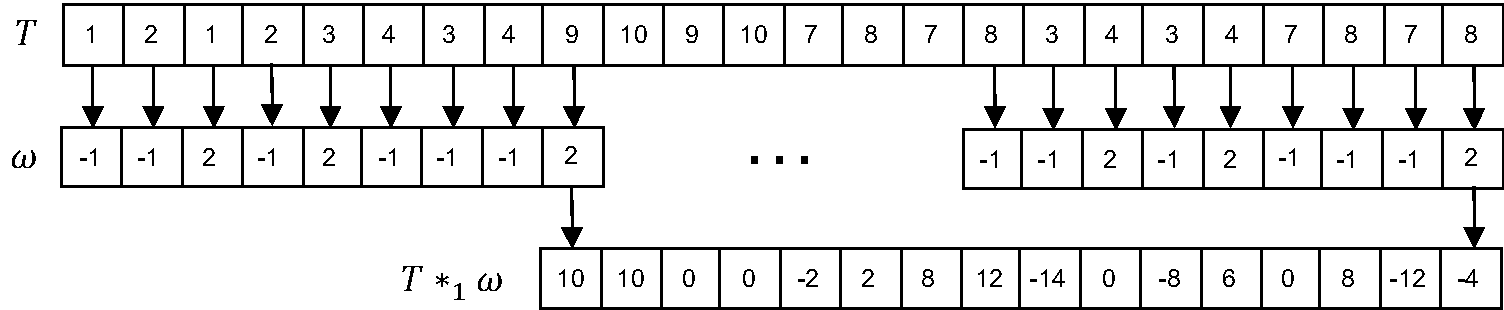
\includegraphics[width=\linewidth]{Figures/conv_d1.pdf}
      \caption{Dilation $d = 1$.}
      \label{fig:conv_d1}
    \end{subfigure}
    \begin{subfigure}{\linewidth}
        \centering
          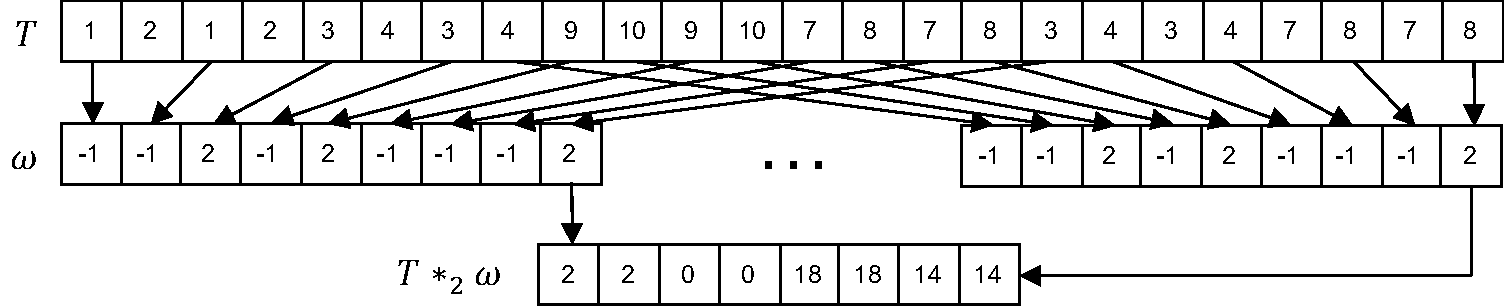
\includegraphics[width=\linewidth]{Figures/conv_d2.pdf}
        \caption{Dilation $d = 2$.}
        \label{fig:conv_d2}
    \end{subfigure}
    \caption{Convolutions with dilations (a) $d = 1$ and (b) $d = 2$.}
    \label{fig:convolutions}
\end{figure}

Let $\Omega = \langle\omega_1, \omega_2, \ldots, \omega_N\rangle \in \mathbb{R}^{N\times m}$ be an ordered sequence of kernels. Each kernel is convolved with $T$ using a discrete set of dilation values $D \subset \mathbb{N}^+$ to produce an ordered set of feature maps $T * \Omega = \langle T*_d\omega_i| 1 \leq i \leq N, d \in D\rangle$.% \in \mathbb{R}^{\left|D\right| \times N \times (n-m+1)}$. 

A \textbf{reduction} function $f: \mathbb{R}^{n-m+1} \rightarrow \mathbb{R}$ computes a scalar property of a feature map; Section \ref{sec:Reductions} lists the reduction functions commonly used for time series classification. 
A \textbf{pooling layer} computes the reduction for each feature map: $F(T * \Omega) = \langle f(T*_d\omega_i)| 1 \leq i \leq N, d \in D\rangle$, % \in \mathbb{R}^{\left|D\right| \times N}$
 producing a \textbf{feature vector} for an independently trained classifier. This approach generalizes to multiple independent reduction functions $f_1, f_2, \ldots, f_M$ which can be concatenated to form a feature vector $F_1(T * \Omega) \cdot F_2(T * \Omega) \cdot \ldots \cdot F_M(T * \Omega)$. %$ \in \mathbb{R}^{\left|D\right| \times N \times M}$.  
Recommended classifiers are \textbf{ridge regression} (for smaller datasets) and \textbf{logistic regression} (for larger datasets) \cite{Rocket}.

\subsection{Dilations}
\label{sec:Dilations}

Computing a convolution using the same kernel but with different dilations can capture the pattern represented by the kernel at varying scales\footnote{
Dilation effectively downsamples $T$ before computing the convolution.
}\footnote{
In a CNN, dilation increases exponentially with network depth. This is not the case with convolutional kernels as discussed here. 
}.  Increasing the dilation value reduces the number of data points in the resulting feature map. 

Dilations that are commonly used in time series classification include: (1) random dilations; (2) uniformly spaced dilations in the range $[1, \lfloor 2^p \rfloor]$, where $p = log_2(n-1)/8$, effectively stretching the maximum length of the largest dilated kernel to $n$ evenly-spaced points spanning the length of the time series; and (3) exponential dilations $\{2^0, 2^1, 2^2, \ldots \}$.

\subsection{Reduction Functions}
\label{sec:Reductions}

Let $T * \omega = \langle u_1, u_2, \ldots, u_{n-m+1} \rangle$. The \textbf{MAX} reduction function is defined as follows:
\begin{equation}
    MAX(T*\omega) = \max\limits_{1 \leq i \leq n-m+1}(u_i \in T*\omega),
    \label{eq:max}
\end{equation}

Four additional reduction functions, defined below, include a \textbf{bias} term $b > 0$, i.e., $T * \omega - \textbf{b} > 0$, or, equivalently, $T * \omega > \textbf{b}$, where $\textbf{b} = \{b\}^{n-m+1}$. The \textbf{(multi-)set of positive values} of convolution $T * \omega$ with bias $b$ is given by:
\begin{equation}
    PV_b(T * \omega) = \underset{1 \leq i \leq n-m+1}{\{ u_i \in T*\omega|u_i > b \}}
    \label{eq:pv}
\end{equation}

The \textbf{Proportion of Positive Values (PPV)} is
\begin{equation}
    PPV_b(T*\omega) =\frac{1}{n-m+1}\biggl| PV_b(T*\omega)\biggr|.
    \label{eq:ppv}
\end{equation}

The \textbf{Mean of Positive Values (MPV)} is
\begin{equation}
    MPV_b(T*\omega) =\frac{1}{|PV_b(T*\omega)|}\sum_{x_i\in PV_b(T*\omega)} x_i.
    \label{eq:mpv}
\end{equation}


The \textbf{Mean of Indices of Positive Values (MIPV)} is
\begin{equation}
    MIPV_b(T*\omega) = \frac{1}{|PV_b(T*\omega)|}\sum_{i=1}^{n-m+1}\{i|u_i > b\}. 
    \label{eq:mipv}
\end{equation}
if at least one scalar value in $T*\omega$ is positive; otherwise, $MIPV_b(T*\omega) = -1$.
%\begin{equation}
%    MIPV_b(T*\omega) = \\
%    \begin{cases}
%    \frac{1}{|PV_b(T*\omega)|}\sum_{i=1}^{n-m+1} \{i|u_i > b\} & |PV_b(T*\omega)| > 0 \\
%    -1 & |PV_b(T*\omega)| = 0
%    \end{cases},
%\end{equation}
%noting that the MIPV is set to $-1$ if all scalar values in $T*\omega$ are non-positive.

The \textbf{Longest Stretch of Positive Values (LSPV)} is
\begin{equation}
    LSPV_b(T*\omega) = \underset{\forall_{i \leq j \leq k},\ u_j > b}{max}(k-i)+1.
    \label{eq:lspv}
\end{equation}

\begin{figure}[tp]
    \centering
    \includegraphics[width=\linewidth]{Figures/reductions.pdf}
    \caption{Examples of a convolution and reduction values with biases $b=0$ (left) and $b=3$ (right).}
    \label{fig:reductions}
\end{figure}

Fig. \ref{fig:reductions} shows examples of the aforementioned reduction functions applied to the convolution shown in Fig. \ref{fig:conv_d2}. 

%\begin{equation}
%    PPV(T*\omega) =\frac{1}{n-m+1}\biggl| \underset{1 \leq i \leq n-m+1}{\{x_i \in T*\omega|x_i > b\}}\biggr|,
%\end{equation}
%\begin{equation}
%    MPV(T*\omega) =\frac{1}{n-m+1}\Sigma\biggl| \underset{1 \leq i \leq n-m+1}{\{x_i \in T*\omega|x_i > b\}}\biggr|.
%\end{equation}

\subsection{Convolutional Kernel-based Classifiers}
\label{sec:Classifiers}

\subsubsection{\textbf{Rocket}}
The \textbf{R}and\textbf{O}m \textbf{C}onvolutional \textbf{KE}rnel \textbf{T}ransform classifier  is parameterized with kernel lengths $m \in \{7, 9, 11\}$, random kernels $\omega \sim \{\mathcal{N}(0,1)\}^{n-m+1}$, and bias $b \sim \mathcal{U}(0,1)$, and random dilation and random padding. Rocket uses the MAX and PPV reduction functions to generate $\mathtt{\sim}20,000$ features: $F_{MAX}(T * \Omega) \cdot F_{PPV}(T * \Omega)$ \cite{Rocket}.  

\subsubsection{\textbf{MiniRocket}}
A simplification of Rocket that achieves comparable accuracy using kernel length $m = 9$, kernels $\omega \in \{-1, 2\}^9$ with the restriction that six values in $\omega$ are $-1$ and three are $2$ (i.e., $C(9, 3) = 84$ kernels), bias $b$ taken from the convolution output, fixed padding and dilation, and uniformly-spaced dilutions, with a maximum number of $32$ dilutions per kernel\footnote{ Less than 32 dilutions per kernel may be appropriate for short time series. 
}. MiniRocket uses the PPV reduction function exclusively to generate $\mathtt{\sim}10,000$ features: $F_{PPV}(T * \Omega)$.

\subsubsection{\textbf{MultiRocket}}
An enhancement to MiniRocket that achieves higher classification accuracy while computing $\mathtt{\sim}5\times$ more features \cite{MultiRocket}. MultiRocket uses similar parameters as MiniRocket, but computes convolutional kernels for time series $T$ and its first-order difference series $T'$, and employs four pooling operators generating $\mathtt{\sim}50,000$ features: $F_{PPV}(T * \Omega) \cdot F_{MPV}(T * \Omega) \cdot F_{MIPV}(T * \Omega) \cdot F_{LSPV}(T * \Omega) \cdot F_{PPV}(T' * \Omega) \cdot F_{MPV}(T' * \Omega) \cdot F_{MIPV}(T' * \Omega) \cdot F_{LSPV}(T' * \Omega)$. 

\begin{figure*}[t]
\centering
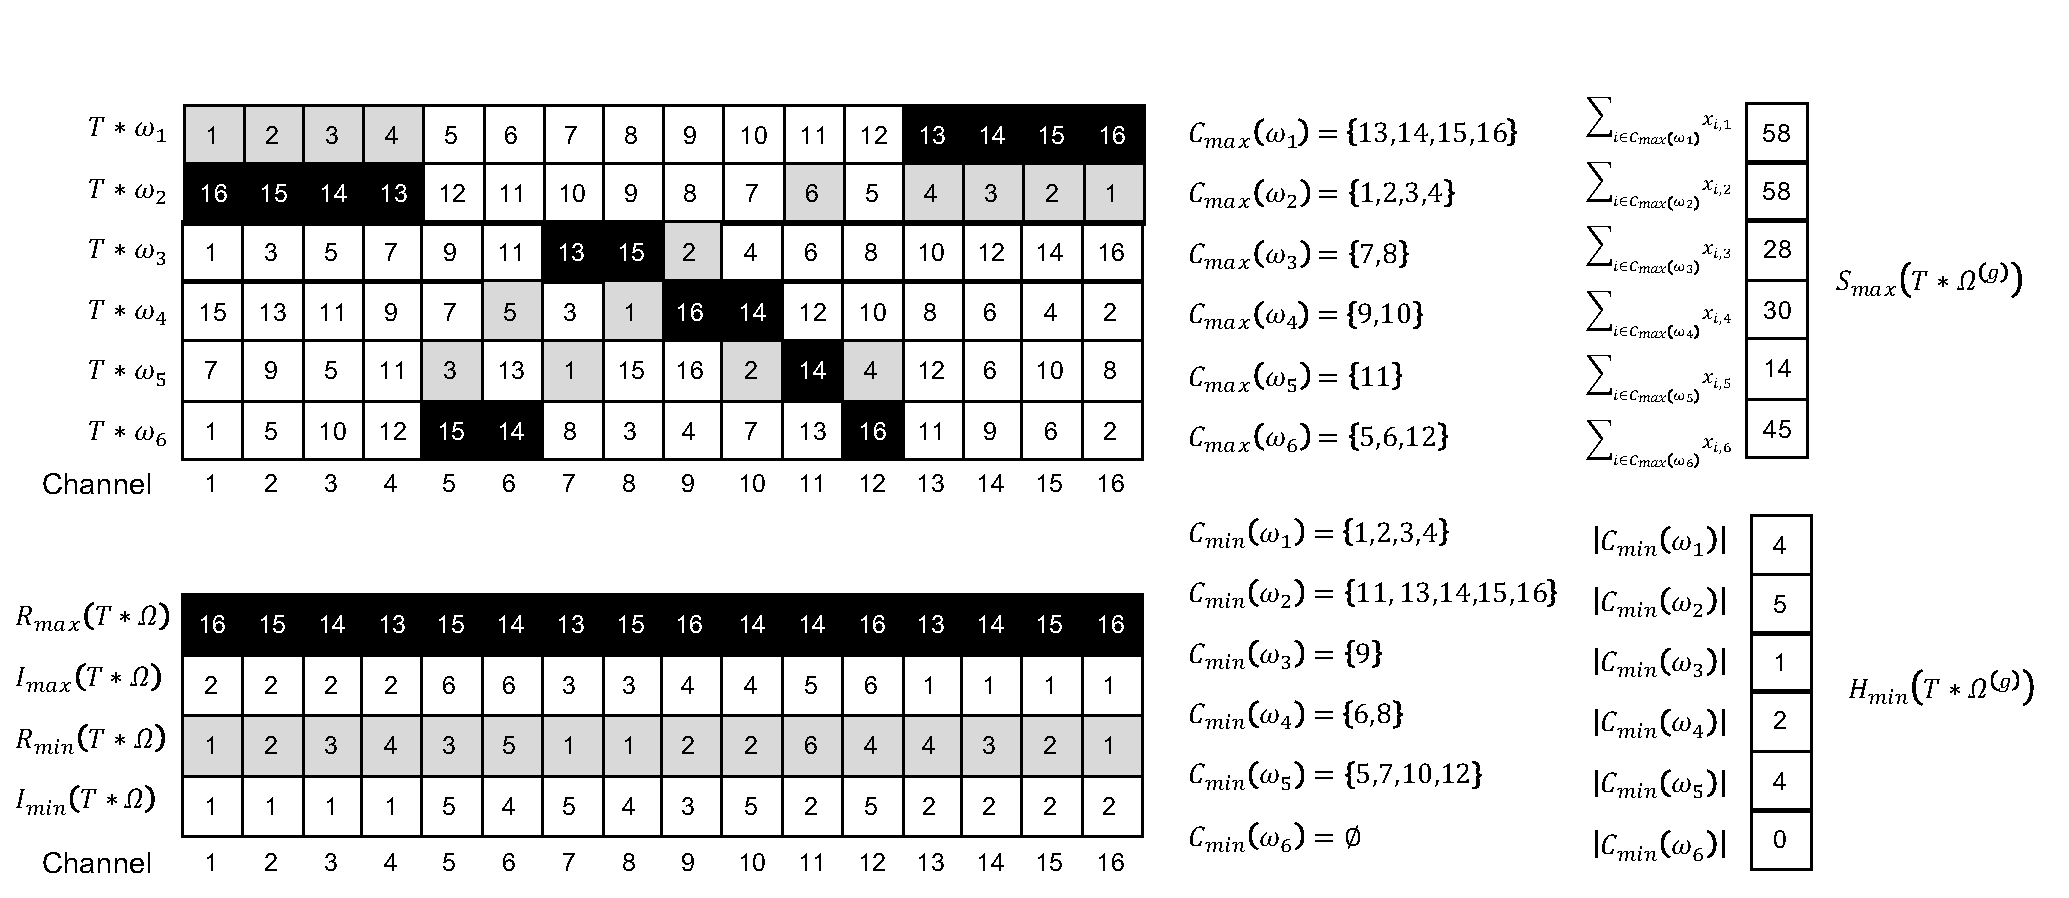
\includegraphics[width=1\linewidth]{Figures/Hydra_counts.pdf}
\caption{Example of Hydra's feature set computed for a single group with $K = 6$ kernels and $p = 16$ channels. When computing maximum/minimum responses per channel, ties go to the entry with the smallest kernel index.}
\label{fig:hydra_counts}
\end{figure*}

\subsubsection{\textbf{Hydra}}
An alternative approach to convolution kernel-based time series classification that computes histograms as features rather than pooling, and achieves higher classification accuracy than Rocket, MiniRocket, and Multirocket.  Hydra computes convolutions for time series $T$ and its first-order difference series $T'$ using kernel length $m = 9$, random kernels $\omega \sim \{\mathcal{N}(0,1)\}^{n-m+1}$, fixed padding, and exponential dilations; Hydra's histograms eschew the need for a bias term. 

Hydra forms $G$ groups of kernels with $K$ kernels per group. Let $\Omega^{(g)} = \langle \omega_1^{(g)}, \omega_2^{(g)}, \ldots, \omega_K^{(g)} \rangle$ denote the $g^{th}$ kernel group. Let $D$ be the set of dilutions. Hydra computes convolutions $T *_d \Omega^{(g)}$ and $T' *_d \Omega^{(g)}$ for all $d \in D$ for the $g^{th}$ group.

Consider convolution $T *_d\ \omega_j^{(g)} = \langle x_{1, j}^{(g)}, x_{2, j}^{(g)}, \ldots, x_{p, j}^{(g)} \rangle$. Larger dilation values $d$ yield shorter convolution lengths $p$. Indices $\langle 1, 2, ... p \rangle$ are called the convolution \textbf{channels}. 

Fig. \ref{fig:hydra_counts} depicts the steps Hydra's feature set computation, described below, for a single group (superscripts $^{(g)}$ omitted for clarity) with $K = 6$ kernels and $p = 16$ channels.  

The \textbf{maximum response} and \textbf{maximum response index} for channel $i$ within group $g$ are respectively computed as:
\begin{equation}
    \mathcal{R}_{max,i}(T *_d \Omega^{(g)}) = \max\limits_{1 \leq k \leq K}(x_{i,k}^{(g)}),
    \label{eq:Rmax}
\end{equation}
and
\begin{equation}
    \mathcal{I}_{max,i}(T *_d \Omega^{(g)}) = \argmax\limits_{1 \leq k \leq K}(x_{i,k}^{(g)}). 
    \label{eq:Imax}
\end{equation}
The \textbf{maximum channel set} for kernel $\omega_j^{(g)}$ is the set of channels for which $\omega_j^{(g)}$ yields the maximum response, i.e.: 
\begin{equation}
    \mathcal{C}_{max}(\omega_j^{(g)}) = \{i|\ \mathcal{I}_{max,i}(T *_d \Omega^{(g)}) = j\}. 
    \label{eq:Cmax}
\end{equation}
\textbf{Minimum} responses, response indices, and channel sets are defined analogously, and correspond to the maximum responses, response indices, and channel sets for the negated kernel set $-\Omega^{(g)} = \langle -\omega_1^{(g)}, -\omega_2^{(g)}, \ldots, -\omega_K^{(g)} \rangle$. 

Hydra defines a \textbf{hard count} as the number of channels for which each kernel computes the maximum response, and a \textbf{soft count} as the sum of maximum responses corresponding to each kernel's hard count. With \textbf{clipping}, Hydra optionally omits negative maximum values and positive minimum values from the counts; clipping is equivalent to passing convolutions through a ReLU function before computing the histograms. 

Hydra computes a \textbf{minimum hard count histogram} and \textbf{maximum soft count histogram} for each group $g$:
%\begin{equation}
%    H_{max}(T *_d \Omega^{(g)}) = \langle |\mathcal{C}_{max}(\omega_j^{(g)})|\ |\ 1 \leq j \leq p \rangle
%\end{equation}
\begin{equation}
    H_{min}(T *_d \Omega^{(g)}) = \left\langle \biggl|\mathcal{C}_{min}(\omega_j^{(g)})\biggr|\ |\ 1 \leq j \leq p \right\rangle 
    \label{eq:Hmin}
\end{equation}
%Hydra's \textbf{maximum/minimum soft count histograms} for group $g$ are computed as follows:
\begin{equation}
    S_{max}(T *_d \Omega^{(g)}) = \left\langle \sum_{i\in \mathcal{C}_{max}(\omega_j^{(g)})}x_{i,j}^{(g)}\ |\ 1 \leq j \leq p \right\rangle
    \label{eq:Smax}
\end{equation}
%\begin{equation}
%    S_{min}(T *_d \Omega^{(g)}) = \left\langle \sum_{i\in \mathcal{C}_{min}(\omega_j^{(g)})}x_{i,j}^{(g)}\ |\ 1 \leq j \leq p \right\rangle
%\end{equation}
Hydra generates the following feature set for downstream classifiers: 
$H_{min}(T *_d \Omega^{(g)}) \cdot S_{max}(T *_d \Omega^{(g)}), 1 \leq g \leq G, d \in D$.

\subsection{Regression Classifier}
\label{sec:regression}

Let $F(T*\omega) \in \mathbb{R}^{\left|D\right| \times N \times M}$ be the feature vector produced by one of the kernel-based classifiers, which is provided as input to an independently trained classifier, either ridge regression for smaller datasets or logistic regression for larger datasets \cite{Rocket}. Both ridge regression and logistic regression are linear classifiers with response function 
$F(T*\omega)\cdot W \in \mathbb{R}$, where $W \in \mathbb{R}^{\left|D\right| \times N \times M}$ is the set of trained weights. 

Let $C = \langle C_1, C_2, \ldots C_P\rangle$ be the set of classes. The regression classifier comprises $P$ independent linear classifiers with weights $\langle W_1, W_2, \ldots, W_P \rangle \in \mathbb{R}^{P\times\left|D\right| \times N \times M}$, each of which predicts the probability that time series $T$ belongs to each of the respective classes. Given a feature vector, the predicted class $C_j$ has the maximum probability, i.e.,
\begin{equation}
    j = \argmax\limits_{1 \leq i \leq P}(F(T*\omega)\cdot W_i). 
    \label{eq:predicted_class}
\end{equation}



%\subsubsection{Arsenal}
%The \textbf{Arsenal} is an ensemble of Rocket classifiers which uses a majority vote to make classification decisions \cite{HIVE-COTE2.0}. The diversity of each Rocket classifier within Arsenal is primarily achieved due to variation among random kernels in each classifier. Ensembles of MiniRocket or MultiRocket classifiers would not make sense because the same set of kernels would be used each time; however, we note that an ensemble of classifiers in which each classifier imposes a different restriction on the values that $\omega$ might take (other than $\{-1, 2\}^9$ could be feasible. Ensembles of Hydra classifiers are possible, but to the best of our knowledge, have not been investigated to date. 